\section{HPC for simulation and simulation for HPC}

Nowadays, many scientific domains rely on simulation in order to better
understand the world around us, or to design systems that are difficult to
prototype and test in the real world. There are many examples of such models, as
can be seen on Figure~\ref{fig:1_introduction:plane} which shows an application
of Computational Fluid Dynamics to model the airflow around a BAE-HAWK plane, or
on Figure~\ref{fig:1_introduction:aevol}, which illustrates the Aevol model, a
digital genetics platform designed to study the evolutionary
process~\cite{aevol}.

\begin{figure}[!ht]
    \centering
    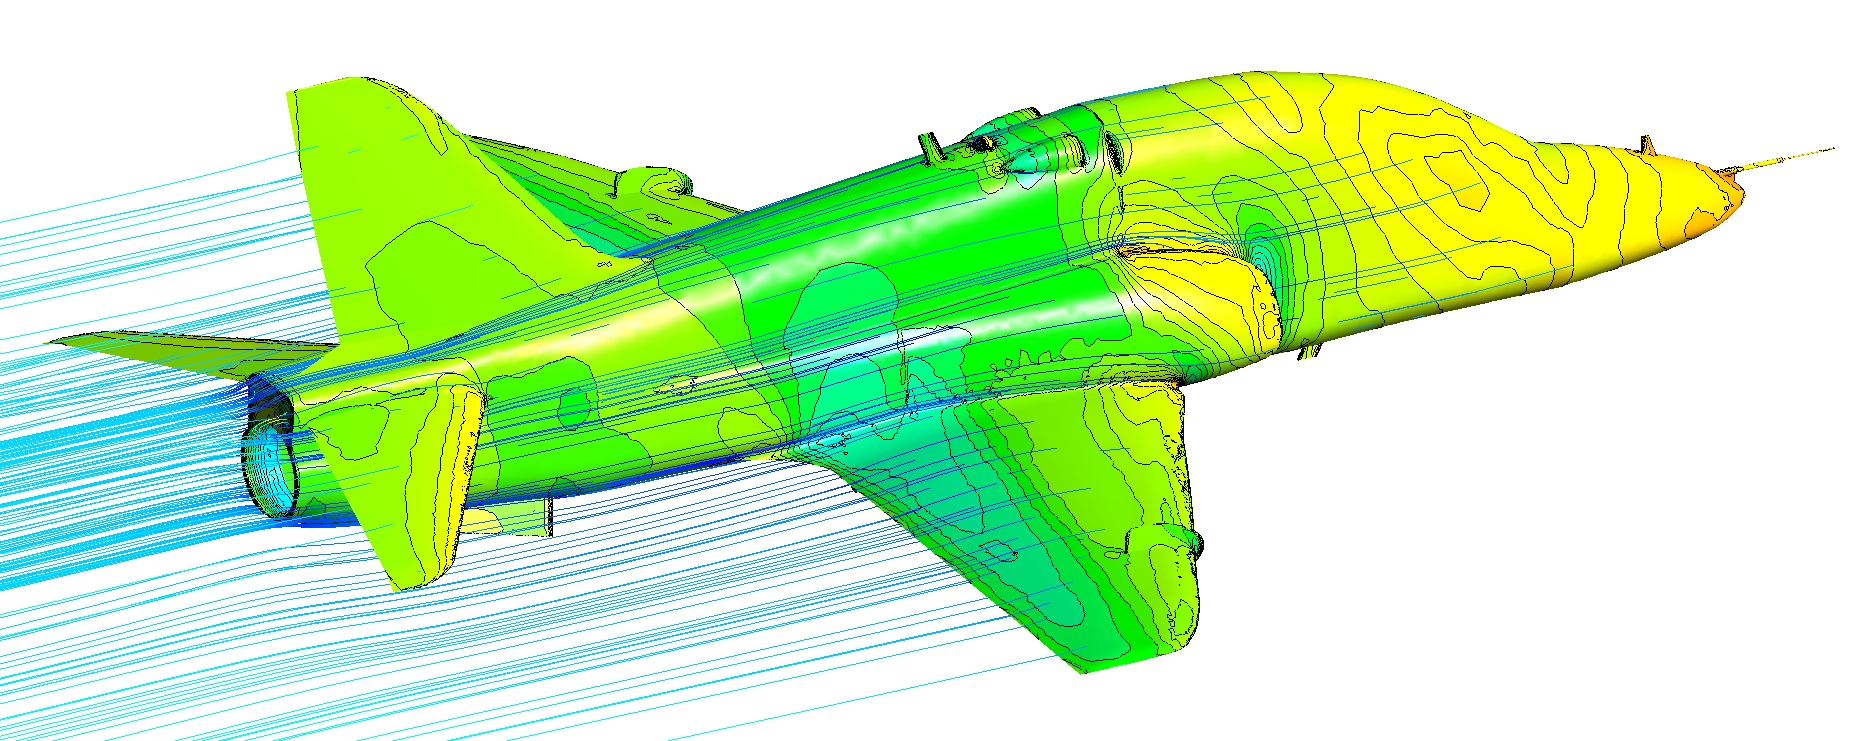
\includegraphics[width=0.7\textwidth]{1_introduction/cfd_plane.png}
    \caption[Fluid dynamic on a BAE-HAWK plane]{Fluid dynamics on a BAE-HAWK plane\protect\footnotemark}
    \label{fig:1_introduction:plane}
\end{figure}

\footnotetext{Image from \url{https://cfd2012.com/aircraft-design.html}}

\begin{figure}[!ht]
    \centering
    
\includegraphics[width=0.9\textwidth]{1_introduction/aevol.png}
    \caption[The Aevol model]{The Aevol model. Image from~\cite{aevol}.}
    \label{fig:1_introduction:aevol}
\end{figure}

As scientific models get more and more accurate, they also become increasingly
complex, and they require an increasing amount of computing power to run. As a
result, most scientific domains today require the use of High Performance
Computing (HPC): clusters of an ever-growing number of machines which work
together towards the same goal. HPC is such a powerful tool that it is used in
most research fields, but also most industries, with applications as varied as
healthcare, weather forecast, geology, every vehicle's design, etc. An example
of such computing cluster is displayed on Figure~\ref{fig:1_introduction:ECMWF},
where we can see the supercomputing facility of the European Centre for
Medium-Range Weather Forecasts (ECMWF) in Bologna, which is made up of Atos
BullSequana XH2000 clusters and is used to run a global Earth system model, in
order to get weather reports as accurate as possible. Additionally, as
artificial intelligence takes an increasing space in our lives, through a huge
diversity of algorithms, the amount of data that we need to process is growing
at a very high rate, and the computing power required to train algorithms
increases proportionally.

\begin{figure}[!ht]
    \centering
    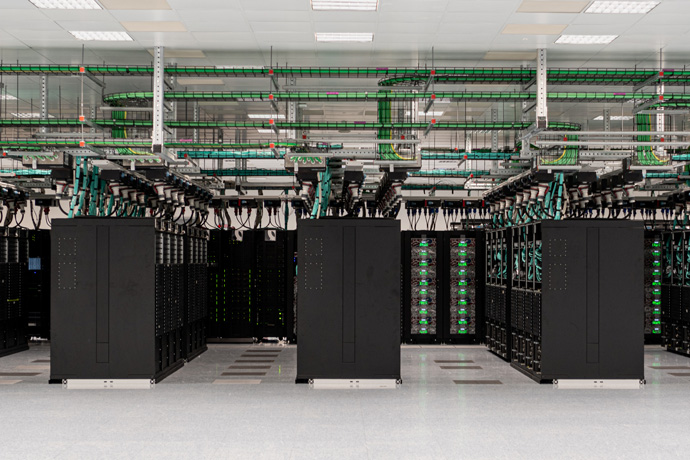
\includegraphics[width=0.7\textwidth]{1_introduction/ECMWF.jpg}
    \caption[HPC facility at ECMWF, made up of four Atos BullSequana XH2000 clusters]{HPC facility at ECMWF, made up of four Atos BullSequana XH2000 clusters\protect\footnotemark}
    \label{fig:1_introduction:ECMWF}
\end{figure}

\footnotetext{Image from \\
\url{https://www.ecmwf.int/en/about/media-centre/focus/2022/fact-sheet-supercomputing-ecmwf}}

As clusters get larger and larger, interconnection networks that connect the
machines together need to handle huge quantities of communications, with the
highest performance possible, in order not to slow down the scientific
applications running on the cluster. In this context, Atos develops its own
interconnection network, the Bull eXascale Interconnect (BXI), which is used in
some of the most powerful European supercomputers, such as
Tera-1000-2~\cite{top500_tera1000} which was the most powerful supercomputer in
Europe at the time of its installation.

Because of the growing complexity of the hardware that is used to power
supercomputers (CPUs, accelerators, interconnection network, etc.), predicting
the execution time of a scientific application on a given cluster is a difficult
task, although it is important for several reasons: for example to dimension new
clusters, or to tune the parameters of the software stack and of the hardware to
optimize performance. Additionally, designing next-generation hardware is
increasingly hard, as we constantly aim for better performance, therefore
conducting studies in simulation is a good tool to facilitate this design
process. This is where simulation can help, by providing a model of the cluster
which can be used to estimate its performance in various scenarios, even
hypothetical ones that cannot be reproduced with the hardware currently
available. This typically happens in the context of the co-design of
next-generation hardware. 

It is important to note that, since the application being run is usually itself
a physical simulation, the word ``simulation'' can be used in this context to
refer to two different objects: the simulation of a supercomputer, which uses
the cluster as the object of its study, and the simulation that might run inside
the cluster, which models a completely different system (as presented
previously). In the context of our work, our contribution is the design of a
simulator of HPC clusters (with a focus on the simulation of BXI), but in order
to validate our model we will also manipulate physics models (presented in
Chapter~\ref{chap:context_hpc}), which we will run in a virtual cluster in the
simulated world. In order to differentiate both types of simulators, in this
document we will refer to physics models as ``scientific applications'' or
``user applications'', to avoid potential confusion with our model of BXI.

In the field of cluster simulation, many types of models are available, which
are used to simulate various parts of a cluster with a high accuracy, or model
the whole cluster, but with a more simplistic model. Our work is a collaboration
between the ``Laboratoire de l'Informatique du Parallélisme'' (LIP) and
Atos\footnote{This PhD is funded by a ``Convention industrielle de formation par
la recherche'' (Cifre)}. In this context, we focus on the communication aspect
of supercomputers, and in particular on the BXI Interconnect made by Atos. Our
model of this hardware is based on the SimGrid framework, which allows us to
design a simulator modeling communications at message-level by leveraging
SimGrid's actor-based flow-model.

In the next section, we will present how BXI is designed at Atos, using our
hands-on experience with this interconnect, the knowledge that we gained from
working inside the low-level software team of this company, and our interactions
with the hardware and high-level software teams. In particular, we will present
the existing uses of simulation in this context, and illustrate the potential
benefits of a more abstract simulator.

\section{Design process of a NIC for HPC at Atos}

The process of creating an Application Specific Integrated Circuit (ASIC), such
as a Network Interface Controller (NIC) in the context of High Performance
Computing, is very costly: the full design and manufacturing process can cost
millions of Euros. Every step of the process is complex, very time-consuming and
expensive, from the design by an R\&D team, to the prototyping, and then the
actual production of the finished product. This is why this creation process
(depicted in Figure~\ref{fig:1_introduction:ASIC}) follows many steps that aim
to facilitate and speed up the design, in order for manufacturers to remain
competitive. 

\begin{figure}[!ht]
    \centering
    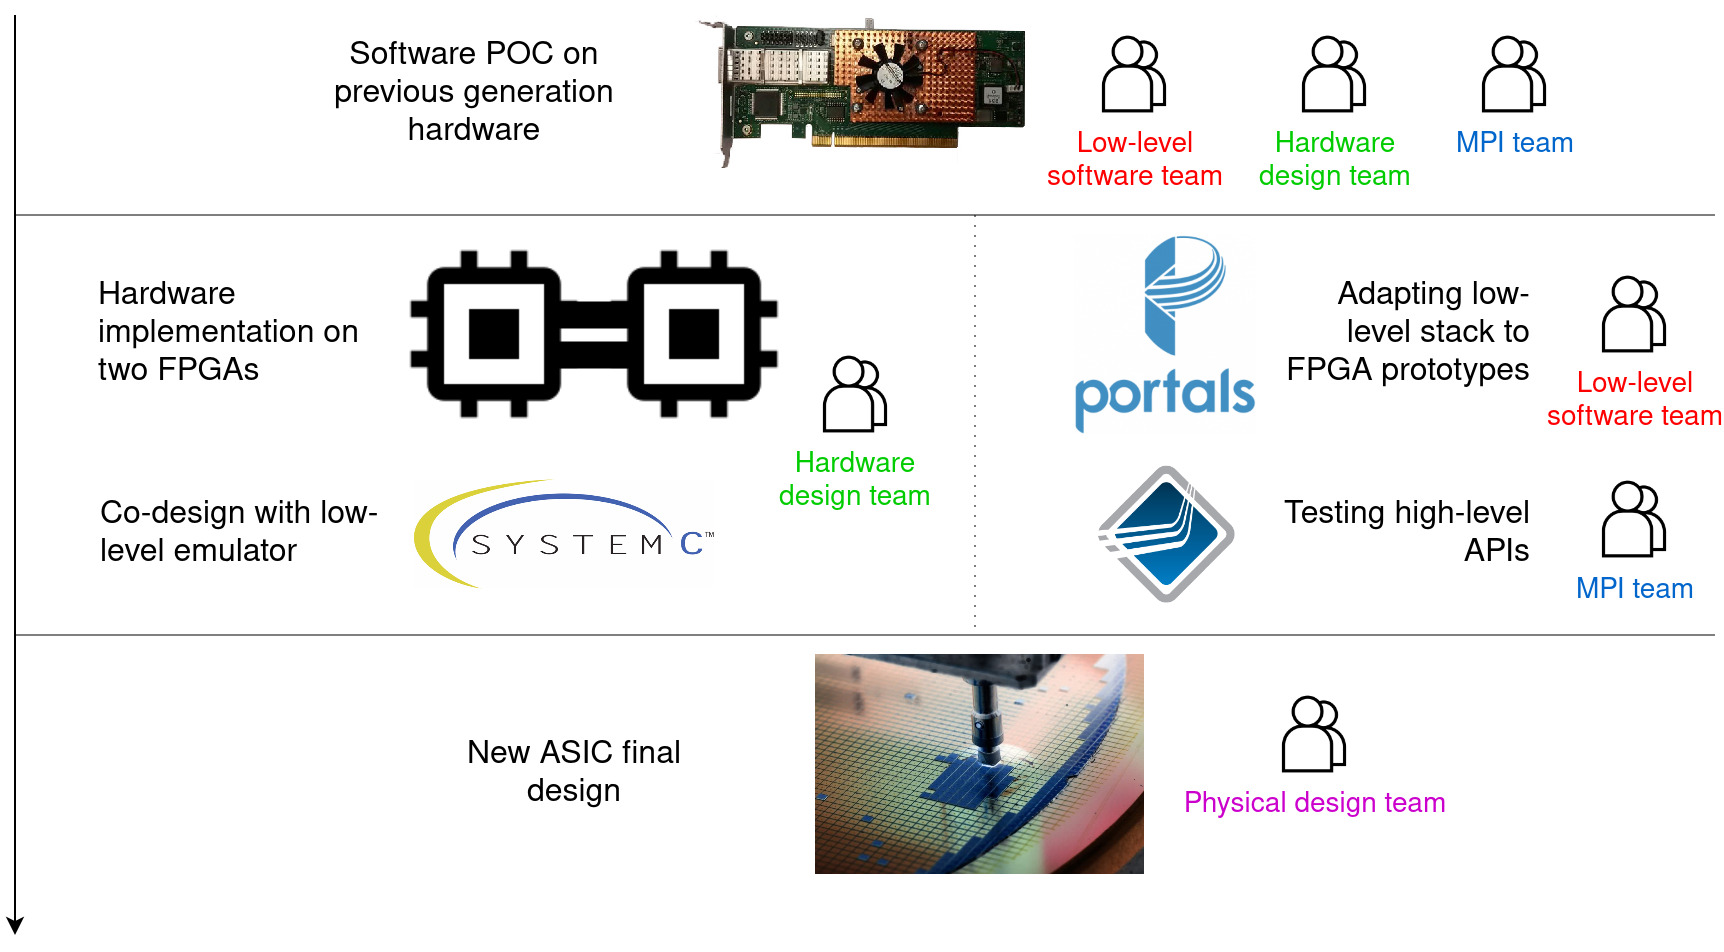
\includegraphics[width=1\textwidth]{1_introduction/ASIC.jpg}
    \caption{Design process of the BXI NIC at Atos}
    \label{fig:1_introduction:ASIC}
\end{figure}

There are mainly four teams that are involved in the process: the hardware
design is made by two teams, which are responsible for the prototyping on
Field-Programmable Gate Arrays (FPGA) and the firmware development on one side,
and the physical layout on the final ASIC on the other side. From the point of
view of the software, there are also two different teams: one of them is
specifically responsible for the tuning of Atos's version of the Message Passing
Interface (MPI), since this high-level API is the most commonly used in the
field of HPC, therefore its maintenance and optimization are very important. The
second team, BXI-LL, is responsible for the lower-levels of the software stack,
which involves developing the driver for BXI NICs, as well as the user-level
library for Portals, which is the network API implemented by the NIC. This API
offers connectionless, reliable point-to-point communications, and since it is
entirely implemented in hardware by the NIC, the user-level software library is
a very thing wrapper that mainly formats commands and sends them to the NIC.
Additionally, the BXI-LL team is responsible for the other high-level services
that are supported by BXI, such as the Lustre distributed Filesystem, OpenSHMEM,
etc.

As we can see on Figure~\ref{fig:1_introduction:ASIC}, the design process of BXI
NICs starts with an exploration of the possible features that could be
implemented, either by emulating these features on hardware that is as similar
as possible to the currently developed ASIC (for example by using old generation
hardware to design the new generation), or using a high-level simulator to get a
rough estimate of the functionality and performance of each option. Once this
step is done and the least promising features have been abandoned, the remaining
ones can be implemented in a first prototype. Because making a physical
prototype would be extremely time-consuming and costly, this step is always done
either on reconfigurable hardware such as an FPGA, or in a very low-level
simulation framework. Sometimes both are made, for example at Atos there is a
SystemC model of the BXI switch, as well as an FPGA implementation.
Additionally, in order to develop the driver and user library for the first
generation of BXI, an emulator of the NIC was made using
QEMU~\cite{bellard2005qemu}, but it was not maintained for the later generation
of BXI hardware. When the first prototype of the hardware is complete, software
developers can start using it to design the driver that is going to power the
hardware. Hardware and software developers then iterate over the prototype to
improve both the circuit and the software stack, until both are ready for
production use, which is assessed with manual tests, as well as the execution of
a test suite designed by the BXI-LL team in order to test most use-cases of the
hardware that need to be supported. At this point, the design on FPGA is passed
to a dedicated team responsible for the layout of the different circuits on the
final chip. Finally, the ASIC is ready to be manufactured at scale.

The issue with this workflow is that a prototype on an FPGA can be around two
orders of magnitude slower than the final product, especially for large circuits
where ``artificial'' bottlenecks can exist on FPGA but not on the final product:
for example the BXI NIC made by Atos does not fit on a single FPGA, and
therefore it is distributed across two FPGAs connected together. Even with this
design, the NIC must be simplified to fit on two FPGAs: only two List Matching
Engines (LMEs) can be implemented instead of four on the real ASIC for example.
These engines are Application-Specific Instruction set Processors (ASIP), which
implement most of the processing of incoming messages, with instructions
optimized to sustain a message rate as high as possible (more details about the
process of receiving messages will be presented in
Section~\ref{subsubsec:4_portals:RX}), therefore having only two on the FPGA
platform instead of four on the final ASIC is a change that has a significant
impact on the behavior of the NIC. With prototypes this slow, it is also
impossible to generate enough traffic to cause meaningful congestion on the
network, which is problematic because congestion is an important phenomenon to
study, as it impacts greatly the performance of networks with real ASICs.
Low-level simulators are even slower than FPGA prototypes, with speeds that are
often several orders of magnitude slower than the final product. This means that
during this development process, software teams can only test their code on very
small scale tests (usually involving two machines at most in the case of NIC
development). This is a problem because it makes it very difficult to evaluate
the performance of the new hardware on a realistic application, which can
exhibit unexpected behavior and performance because of the complex interaction
between all the components of a modern cluster. For example, at a small scale an
application might be CPU-bound, but at a larger scale communications might
become more important and stress the memory, which could become the bottleneck
since it is a shared resource between the CPUs and NICs. This problem becomes
even more complex if a storage system or an accelerator uses the memory at the
same time, or if the data that needs to be sent on the network is on the
storage. All of these scenarios create interdependencies between the different
resources, and their impact on performance at different scales can be
unexpected.

This is why it would be beneficial for the different development teams to have a
model of the new hardware at an intermediate level: more accurate than the
initial rough approximations, but faster than low-level emulators, in order to
study more realistic workloads. The hardware and low-level software team at Atos
could use it to perform studies on specific properties of the hardware, for
example evaluating the impact of different protocol design choices. The teams
responsible for the development of Atos's version of MPI could use it for
higher-level studies, such as tuning the algorithms used by MPI to perform
complex operations between many machines, or testing their developments.
Finally, Atos's clients could use our simulator to evaluate the performance of
their applications, and tune the configuration of their code before performing
real-world executions. In particular, the main client of the BXI Interconnect,
the ``Commissariat à l'Énergie Atomique et aux Énergies Alternatives'' (CEA)
showed interest in our work, and could be a potential user of our simulator.

\section{Contributions}

In our work, we design a simulator of HPC clusters, that is focused on the
simulation of the BXI interconnect made by Atos. As BXI NICs implement the
Portals API in hardware, we propose an implementation of this API in simulation.
To this end, we rely on the SimGrid framework, which provides a flow-model of
communication, and allows us to implement a Discrete Event Simulator (DES) using
cooperative Actors. Even though flow-models are typically used to simulate
communication at message level, we use a novel approach that models transfer at
a lower level of granularity than most state-of-the art simulators. This design
choice allows us to create a more accurate model of the hardware, without
modeling each packet individually. To the best of our knowledge, this is the
first time that a model of Portals has been made publicly available. We validate
our model, using low-level experiments which rely on the Portals API.

We show that our simulation method is versatile, by running high-level network
APIs on top of our low-level model. In this context, we study in detail the
execution of Atos's implementation of MPI in our simulator, and we also show
preliminary work with OpenSHMEM. To validate our model in this context, and to
compare it with the closest state-of-the-art MPI simulator, SMPI, we run
unmodified scientific applications that are commonly used to assess the
performance of HPC clusters. These experiments confirm our expectations, as we
observe that our simulation method is more accurate than SMPI, but also slower,
as our model is more detailed. Therefore, we explore a new method to tune the
ratio between performance and accuracy of our simulation method, by combining
our network model and SMPI's, and enabling users to switch between them at
runtime.

We conduct a study in order to assess the usefulness of potential evolutions of
BXI NICs, by implementing flow-control mechanisms in simulation and testing this
feature in different scenarios. This study shows the versatility of our
simulator, as it demonstrates how low-level features of the hardware can be
evaluated using high-level benchmarks, and we present a few other studies which
could be conducted using a similar methodology (but which are left as future
work).

\section{Structure of this thesis}

Our contributions are organized in seven chapters:
Chapter~\ref{chap:context_hpc} gives context regarding the field of HPC, by
presenting the architecture of a typical HPC cluster and the most significant
interconnection networks. It also details properties of the Portals API which
will be important for the rest of our work, and describes a few scientific
applications which will be used in our experiments.

Chapter~\ref{chap:biblio_simu} presents pre-existing simulators of HPC clusters,
with a focus on SimGrid in order to illustrate the most important features which
we leverage in our simulator. 

Chapter~\ref{chap:low_level} then focuses on our
low-level model, by explaining how Portals is implemented in simulation, and
which properties of the hardware are modeled by our approach. It also shows
validation results by relying on point-to-point benchmarks of Portals. Even
though this work was published in~\cite{Emmanuel2020a}, in this thesis we also
present several features of our simulator which were added after the initial
publication. 

Chapter~\ref{chap:high_level} explains how this model can be used to run
high-level APIs, and in particular MPI. To this end, it details the
modifications that need to be performed on the real-world implementations of MPI
and OpenSHMEM in use at Atos, in order to make them compatible with our
simulator. Part of this work was published in~\cite{Emmanuel2021}, but
significant work has been added since: in particular, this publication does not
mention our study on OpenSHMEM, and our benchmarks are now more complete.

Chapter~\ref{chap:model_change} shows how we can combine two network models, and
allow users to switch between them at runtime. 

Chapter~\ref{chap:flowctrl}
discusses some ideas that are more experimental, in particular it details our
study on flow-control in BXI (a very early version of this work was published
in~\cite{Emmanuel2021}), and it lists ideas that are left as future work.

Finally, Chapter~\ref{chap:conclusion} concludes this document by summarizing
our work.
